\documentclass[a4paper, 11pt]{article}
\usepackage{comment} % enables the use of multi-line comments (\ifx \fi) 
\usepackage{lipsum} %This package just generates Lorem Ipsum filler text. 
\usepackage{fullpage} % changes the margin
\usepackage{epsfig}
\usepackage{listings}

\begin{document}
%Header-Make sure you update this information!!!!
\noindent
\large\textbf{Lab Report:2} \hfill \textbf{Abhishek Srivastava \& Ravdeep Pasricha} \\
\normalsize CS202 Advanced Operating Systems\hfill Student Id: 861307778 \& 861307836 \\
Prof. Nael B. Abu-Ghazaleh \hfill \today \\
\hrule

\noindent
\\
\large\textbf{Problem}\\

- \textbf{clone()} system call.

- \textbf{thread\_create()} function implementation.

- \textbf{Spin Lock} initialization, acquire and release implementation.

- \textbf{Array based queue Lock} initialization, acquire and release implementation.

- \textbf{Sequential Lock} initialization, acquire and release implementation.

- \textbf{MCS Lock} initialization, acquire and release implementation.

- \textbf{Frisbee} program implementation.\\

\noindent
\large\textbf{Solution}\\

\begin{itemize}
\item Files Modified
\begin{itemize}
\item \textbf{defs.h}: Modified for adding clone system call  \emph{int clone(void *, int);}.
\item \textbf{proc.c}:  Added the definition of \emph{int clone(void* stack, int size)} to create a new process, copy the pagedir of the parent and create a local stack of thread for each thread and copy the content of the parent process. \emph{wait()} and \emph{exit()} system call is also modified to handle the shared data between the threads. It is done by maintaining a thread count and freeing the memory only when a single process/thread is left.
\item \textbf{proc.h}: Modified \emph{proc} data structure to add $ppid$ variable which has the parent process id. It is used to identify the thread who share the same parents. For calculation of the execution time few more parameters are added to the proc structure.
\item \textbf{syscall.h}, \textbf{syscall.c}, \textbf{sysproc.c}, s\textbf{usys.S}, \textbf{user.h}: Modified to add Clone System call.
\item \textbf{Makefile}: Modified for the compilation purposes.
\end{itemize}
\item File added 
\begin{itemize}
\item \textbf{frisbee.c} : Implementation of frisbee program using simple spin lock.
\item \textbf{frisbee\_arr.c}: Implementation of frisbee program using array based queuing lock.
\item \textbf{frisbee\_seq.c}: Implementation of frisbee program using sequential lock.
\item \textbf{frisbee\_mcs.c}: Implementation of frisbee program using mcs lock.
\item \textbf{libthread.h}: Contains the definition of all the locks and thread calls.
\item \textbf{libthread.c}: Contains the implementation of all the lock calls for initialization, acquire and release.
\end{itemize}

\item Functions and System calls added\\
\textbf{Clone System call in proc.c}


\begin{lstlisting}
int
clone(void* stack, int size)
{
    int i, pid;
    struct proc *np;
    
    // Allocate process.
    if((np = allocproc()) == 0){
        return -1;
    }

    //cs202: use the same address space as parent
    np->pgdir = proc->pgdir;
    np->sz = proc->sz;
    np->parent = proc;
    *np->tf = *proc->tf;
    //cs202: assigning parent id
    np->ppid = proc->pid;
    proc->thread_count++;
    // Clear %eax so that fork returns 0 in the child.
    np->tf->eax = 0;
    //cs202: calculating esp location in current stack
    //which is also the stack size
    uint esp_addr = *(uint*)proc->tf->ebp - proc->tf->esp;
    //cs202: calculating ebp locatoin in current stack
    uint ebp_addr = *(uint*)proc->tf->ebp - proc->tf->ebp;
    //cs202: set esp value of created thread 
    np->tf->esp = (uint)stack + size - esp_addr;
    //cs202: set ebp value of created thread
    np->tf->ebp = (uint)stack + size - ebp_addr;

    //cs202: copying the stack content from current process
    memmove((void *)np->tf->esp, (void *)proc->tf->esp, esp_addr);
    for(i = 0; i < NOFILE; i++)
        if(proc->ofile[i])
            np->ofile[i] = filedup(proc->ofile[i]);
    np->cwd = idup(proc->cwd);
    safestrcpy(np->name, proc->name, sizeof(proc->name));
    pid = np->pid;
    acquire(&ptable.lock);
    np->state = RUNNABLE;
    release(&ptable.lock);
    return pid;
}
\end{lstlisting}

\textbf{Locks defintion added in libthread.h}
\begin{lstlisting}
//cs202
//spin lock
struct lock_t {
     //store the lock value if 0 then not locked, if 1 then locked
    uint is_locked;
};


//spin lock calls implementation
void lock_init(struct lock_t* l);
void lock_acquire(struct lock_t* l);
void lock_release(struct lock_t* l);

//array lock
struct alock_t {
    uint *lock_array; 	//lock array
    uint num_th; 	//number of threads
    uint next_slot; 	//next slot id
    uint curr_slot;	//current slot id
};

//array lock calls implementation
void alock_init(struct alock_t* l, uint num_t);
void alock_acquire(struct alock_t* l, int tid);
void alock_release(struct alock_t* l);
int fetch_and_increment(uint* next);

//sequential lock
struct seqlock_t {
    uint seq_counter;
    struct lock_t sl;
};

//seq lock calls implementation
void seqlock_init(struct seqlock_t* l);
void write_lock(struct seqlock_t* l);
void write_unlock(struct seqlock_t* l);
uint read_counter(struct seqlock_t* l);

//mcs lock
struct mcslock_node {
    uint is_locked;
    struct mcslock_node *next;
};

//mcs lock node
struct mcslock_t {
    struct mcslock_node* node;
};

//mcs lock calls implementation
void mcslock_init(struct mcslock_t* l);
void mcslock_nodeinit(struct mcslock_node* n);
void mcslock_acquire(struct mcslock_t* l, struct mcslock_node* n);
void mcslock_release(struct mcslock_t* l, struct mcslock_node* n);
struct mcslock_node* fetch_and_store(struct mcslock_t* l, 
				struct mcslock_node* n);

//thread calls
int thread_create(void* (*start_routing)(void *) , void *);
int thread_join(void);

\end{lstlisting}

\textbf{Implementation of locks calls in libthread.c}
\begin{lstlisting}
#include "types.h"
#include "user.h"
#include "stat.h"
#include "x86.h"
#include "libthread.h"

//spin lock calls
void lock_init(struct lock_t* l) {
    l->is_locked = 0;
}

void lock_acquire(struct lock_t* l) {
    while(xchg(&l->is_locked, 1) != 0);
}

void lock_release(struct lock_t* l) {
    if(l->is_locked)
        xchg(&l->is_locked, 0); 
}

//array lock calls
void alock_init(struct alock_t* l, uint num_t) {
    //memory allocation for array lock
    uint *arr = malloc(sizeof(uint) * num_t);
    //intialization
    l->lock_array = arr;
    int i;
    for(i=0; i<num_t; i++)
        l->lock_array[i] = 0;
    l->lock_array[0] = 1;

    l->num_th = num_t;
    l->next_slot = 0;
    l->curr_slot = -1;
}

void alock_acquire(struct alock_t* l, int tid) {
    while( l->lock_array[tid] != 1);
    l->curr_slot = tid;
    l->next_slot = l->curr_slot + 1;
    if(l->next_slot == l->num_th)
        l->next_slot = 0;
}

void alock_release(struct alock_t* l) {
    if( l->lock_array[l->curr_slot] ) {
        l->lock_array[l->curr_slot] = 0;
        l->lock_array[l->next_slot] = 1;
    }
}

int fetch_and_increment(uint *next) {
    xchg(next, *next+1);
    return (*next)-1; 
}

//seq lock calls
void seqlock_init(struct seqlock_t* l) {
    l->seq_counter = 0;
    lock_init(&l->sl);
}

void write_lock(struct seqlock_t* l) {
    lock_acquire(&l->sl);
    l->seq_counter++;
}

void write_unlock(struct seqlock_t* l) {
    l->seq_counter++;
    lock_release(&l->sl);
}

uint read_counter(struct seqlock_t* l) {
    return l->seq_counter;
}

//mcs lock calls
void mcslock_init(struct mcslock_t* l) {
    l->node = 0;
}

void mcslock_nodeinit(struct mcslock_node* n) {
    n->is_locked = 0;
    n->next = 0;
}

void mcslock_acquire(struct mcslock_t* l, struct mcslock_node* n) {
    //Algo/pseudo code from the paper

    struct mcslock_node* pred = fetch_and_store(l,n);
    if(pred != 0) {
        n->is_locked = 1;
        pred->next = n;
        while(n->is_locked); 
    }
}

void mcslock_release(struct mcslock_t* l, struct mcslock_node* n) {
    //Algo from the book
    if(n->next == 0) {
        struct mcslock_node* old_tail = fetch_and_store(l,0);
        if(old_tail == n)
            return; 
        struct mcslock_node* usurper = fetch_and_store(l,old_tail);
        while(n->next == 0);
        if(usurper != 0)
            usurper->next = n->next;
        else
            n->next->is_locked = 0;
    }
    else
        n->next->is_locked = 0;
}

struct mcslock_node* fetch_and_store(struct mcslock_t* l, 
				struct mcslock_node* n) {
    struct mcslock_node* ret_node;
    ret_node = l->node;
    l->node = n;
    return ret_node;
}

//thread interface
int thread_create(void* start_routine(void *), void* arg) {
    uint stack_size = 4096;
    void *stack = malloc(stack_size);
    int t_id = clone(stack,stack_size);
    if(t_id == 0) {
        (start_routine)(arg);
        exit();
    }
    else
        return t_id;
}

int thread_join(void) {
    return wait();
}
\end{lstlisting}

\textbf{Frisbee implementation with Spin Lock}
\begin{lstlisting}
#include "types.h"
#include "stat.h"
#include "user.h"
#include "libthread.h"

//total number of threads to be created
uint num_threads;
//total number of times frisbee to be passed
uint num_pass;

//values related to frisbee
struct frisbee {
    uint token;	//token value
    uint pass_value; //pass value
    struct lock_t sl; //spin lock
} spin;

struct data {
    int tid;
};

//This is the function which threads will be executing
//In this thread we check the token value and if it is same as thread id
//we increase the pass count till number of pass value is less than total number of pass
void* pass_frisbee(void* arg)
{
    struct data *fdata = (struct data *)arg;  

    int thid = fdata->tid; //thread id

    while(spin.pass_value < num_pass) {
        //acquire the lock
        lock_acquire(&spin.sl);
        
        //if token value is same thread id
        if(thid == spin.token && spin.pass_value < num_pass) {
            spin.pass_value++;
            spin.token = spin.token++;
            
            if(spin.token == num_threads)
                spin.token = 0;
            printf(1,"Pass number no: %d, Thread %d is passing the token 
            to thread %d\n", spin.pass_value, thid, spin.token);
        }
        //release the lock
        lock_release(&spin.sl);
    }
    return 0;
}

int main(int argc, char*argv[])
{
    struct data *tdata;
    //check if parameters entered are correct
    if(argc != 3) {
        printf(1,"frisbee <num_thread> <num_pass>");
        exit();
    }
    
    num_threads = atoi(argv[1]);
    num_pass = atoi(argv[2]);
    //spin lock initialization
    //initialize token value
    spin.token = 0;
    spin.pass_value = 0;
    //lock intialization
    lock_init(&spin.sl);
    //create threads
    int i;
    //thread data to pass to the threads
    tdata = malloc(sizeof(struct data) * num_threads);
    for(i=0; i<num_threads; i++)
        tdata[i].tid = i;

    for(i = 0; i<num_threads; i++) {
        thread_create((void*)pass_frisbee,(void*)&tdata[i]);
    }
    //wait for all threads to finish
    for(i = 0; i<num_threads; i++) {
        thread_join();
    }
    printf(1, "\nSpin Lock Demo\n");
    printf(1, "\nSimulation of Frisbee game has finished, 
	    %d rounds were played in total!\n", num_pass);
    return 0;
}

\end{lstlisting}

Similar to this we have implemented Array based queue locking, Sequential locking and MCS locking. We have provided their code 
\emph{frisbee\_arr.c}, \emph{frisbee\_seq.c} and \emph{frisbee\_mcs.c}.
\newpage
\item Result

From the execution of all the lock implementation we can see in the results that spin lock  is the slowest one. Sequential lock(921 ticks) performs way better than Spin lock(3102 ticks) when thread number is in large numbers. Screen shots of the executions of all the locks implemented is attached below with execution time in ticks is also shown in them. 

\begin{figure}[h]
	\centering
	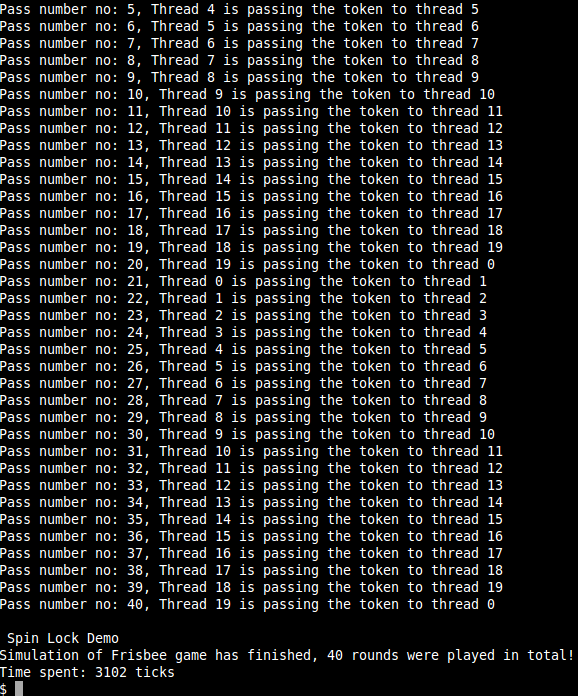
\epsfig{file=L2_SS1.png, height=6in, width=5in}
	\caption{Spin Lock Execution Result.}
\end{figure}

\begin{figure}
	\centering
	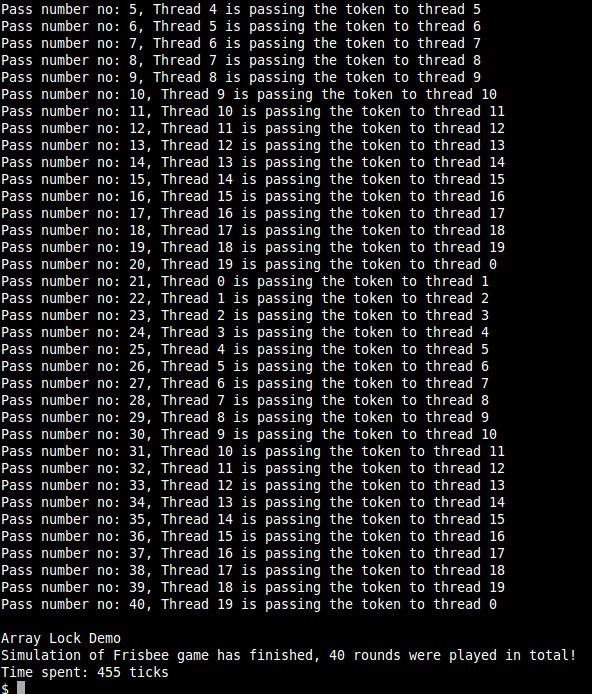
\epsfig{file=L2_SS2.png, height=6in, width=5in}
	\caption{Array Based Queuing Lock Execution Result.}
\end{figure}

\begin{figure}
	\centering
	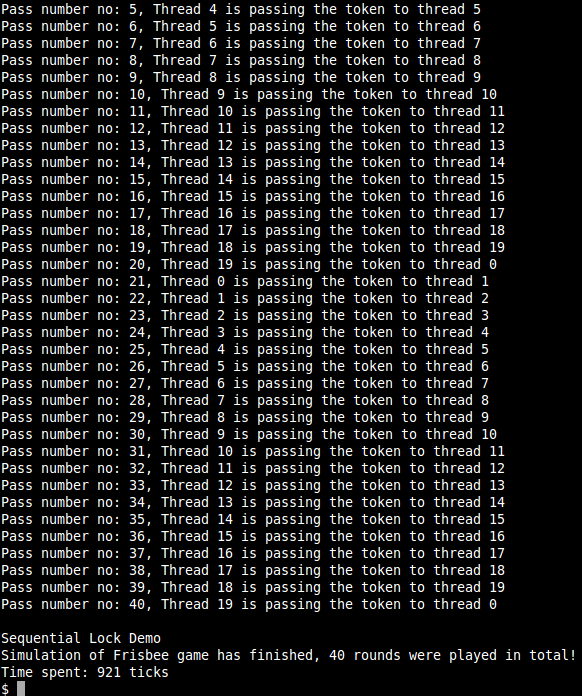
\epsfig{file=L2_SS3.png, height=6in, width=5in}
	\caption{Sequential Lock Execution Result.}
\end{figure}

\begin{figure}
	\centering
	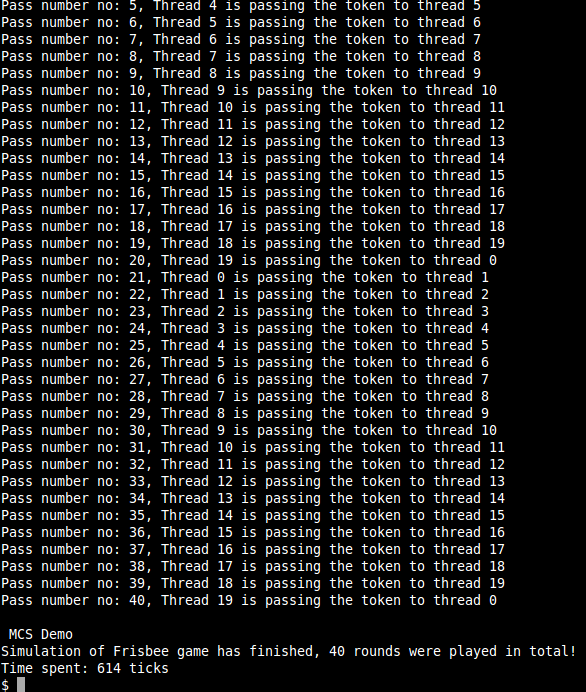
\epsfig{file=L2_SS4.png, height=6in, width=5in}
	\caption{MCS Lock Execution Result.}
\end{figure}

\end{itemize}
\end{document}
